


\chapter{Force Fields and Statistical Potentials}
\label{appendix:force_fields_statistical_potentials}
Many methods developed for model quality assessment use a particular optimization function, called scoring function, with the aim to summarize the most interesting features of a protein model.\\
Scoring functions used by MQAPs are similar to those defined in other fields of bioinformatics such as fold recognition, \emph{ab initio}, protein design, refinement of predicted three-\-di\-men\-sio\-nal protein structure, molecular mechanics or dynamics. Generally, energy functions are classified as follows:
\begin{itemize}
\item Force fields.
\item Statistical potentials.
\end{itemize}
A force field represents a predictive model described by using a physical approach, while a statistical potential builds a statistical model based on the amino acid distribution extracted from a set of known proteins. Generally, force fields are recognized to be more accurate than statistical potentials, although the latter approximate better the distance from the native protein structure (see Figure \ref{fig:energy_minimization}). The following sections examine the details of these categories.
\begin{figure}[tb]
	\begin{center}
		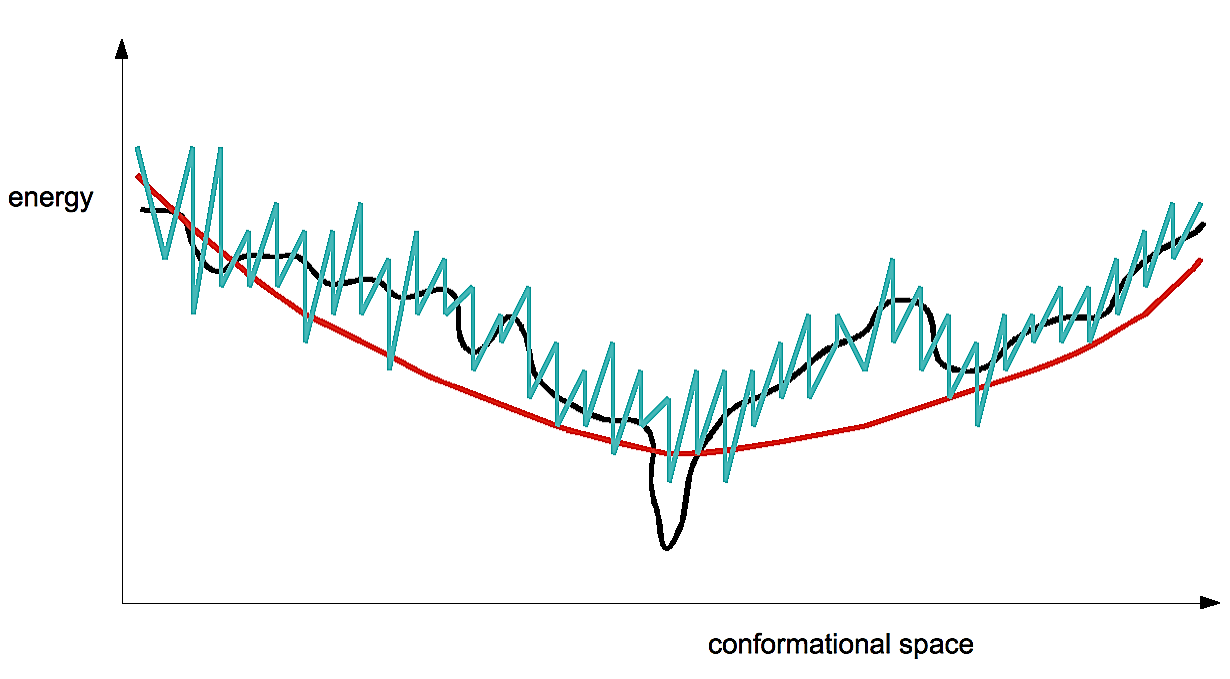
\includegraphics[scale=0.30]{energy_minimization}
		\caption[Example of energy minimization using force fields or statistical potentials]{Example of energy minimization using force fields or statistical potentials. The plot illustrates the differences between force fields and statistical potentials applications in the approximation of the real folding process of a hypothetic protein. Force fields (turquoise line) are more accurate than statistical potential (red line) in capturing the real energy of the protein structure (black line). However, statistical potentials approximate better the distance from the protein native structure that is located in the minimum energy point. A clear problem related to field forces is the presence of many local minima during the search in the conformational space.}
		\label{fig:energy_minimization}
	\end{center}
\end{figure}


\section{Force Fields}
\label{sec:force_fields}
Scoring functions based on force fields are heavily used in molecular mechanics or dynamics and protein design. The global energy of a certain protein conformation is estimated by a linear combination of different energy contributions. These are related to the short, medium and long-range interactions computed on all pairs of atoms that build the system.\\
Historically, this type of function was developed for two reasons:
\begin{description}
\item[Molecular mechanics.] Used to study small molecules as well as large biological systems or material assemblies with many thousands to millions of atoms. An application regards the optimization of three-\-di\-men\-sio\-nal protein structures, obtained experimentally or by a computational method. This is achieved by applying local improvement to the backbone and side chains, reducing collisions and minimizing the energy of the system.
\item[Molecular dynamics.] Simulations in which the target protein is surrounded by a huge number of water molecules, allowing it to evaluate all possible forces existing between atoms of the system. In this way, it is possible to study the movement of the structure in its real environment. 
\end{description}
A basic global energy of the structure is computed by using \emph{bonded terms} and \emph{non-bonded terms} as follows:
\begin{equation}
 	E = E_{bonded} + E_{non-bonded}
\end{equation}
where $E_{bonded}$ is defined as
\begin{equation}
 	E_{bonded} = E_{bond} + E_{angle} + E_{improper} + E_{torsion}
\end{equation}
and $E_{non-bonded}$ as
\begin{equation}
 	E_{non-bonded} = E_{electrostatic} + E_{vanderWaals}
\end{equation}
These contributions are estimated by mathematical functions that relate the force between two atoms to their relative positions. Figure \ref{fig:potential_energy} shows the terms from both graphical and mathematical points of view.\\
\begin{figure}[tb]
	\begin{center}
		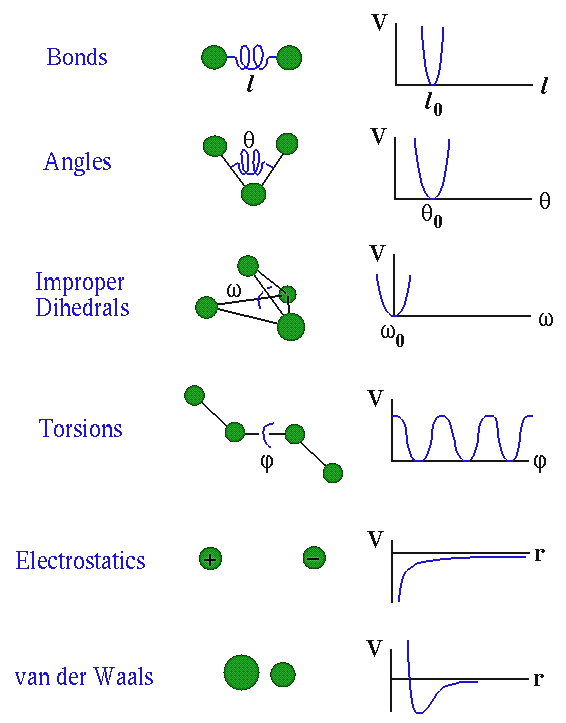
\includegraphics[scale=0.40]{pe}
		\caption[Functions to describe energy terms]{Functions to describe energy terms. $E_{bond}$ and $E_{angle}$, called also bond stretching and angle bending respectively, are described by simple harmonic functions. Harmonic potentials are also used to represent the planarity of some groups. This kind of potential is known as improper dihedrals, $E_{improper}$. Torsion angles are represented by sinusoidal energies, $E_{torsion}.$ The electrostatic attraction or repulsion between two charges is described by Coulomb's law, $E_{electrostatic}$. The Lennard-Jones potential models the attractive and repulsive interactions, $E_{vanderWaals}$. (Source: \href{http://cmm.info.nih.gov/intro\_simulation/node15.html}{http://cmm.info.nih.gov/intro\_simulation/node15.html}).}
		\label{fig:potential_energy}
	\end{center}
\end{figure}
\emph{Bonded terms}, i.e. $E_{bond}$, $E_{angle}$ and $E_{torsion}$, are applied to a set of two to four atoms respectively, that are covalently bonded. The term $E_{improper}$ is used to describe the planarity of some groups, i.e. the amide planes of proteins. These terms describe structural constraints of the protein. The idea is that the larger is the distance between the measured and expected values, the more the scoring function penalizes the protein conformation.
$\emph{Non-bonded terms}$, i.e. $E_{electrostatic}$ and $E_{vanderWaals}$, deal with non covalent bonds between atoms. The former approximates the protein model using dielectric constants dependent on the distance of charged groups with the aim to estimate the Coloumb interactions. The latter studies the variation of the energy in function of the distance between atoms. It includes two components: strong short-ranged repulsive and weak long-ranged attractive. It is used with the intention to reduce structural overlaps. Typically, force fields are computed by considering only physical models and theoretical knowledge, and not based on experimental observation such as the Ramachandran plot. Also, they do not take into account solvation contribution and interactions based on hydrogen bonds.



\section{Statistical Potentials}
\label{sec:statistical_potentials}
Statistical potentials, also called knowledge-based potentials, represent statistical parameters derived from the analysis of a database containing characteristics of known proteins. The key concept underlying statistical potentials is that the information collected from a wide significative dataset should be able to capture empirically some physico-chemical aspects of the protein structure. For instance, by analyzing a huge set of known protein structures, it could be found that some particular amino acids are more involved in the formation of a specific structural pattern, i.e. $\alpha$-helix or a $\beta$-strand, than others. Therefore, if the structural pattern is found in an unknown protein structure, it is reasonable to associate it to the residues considered more involved.\\
Generally, the probabilities are determined by statistical examination of native contacts present in a database of structures represented in the PDB. According to the energy landscape view of protein folding, structures that closely resemble the native state will be distinguishably lower in free energy than those that are different from the native state. These probabilities are converted into pseudo-energies by using equations similar to the Boltzmann law:
\begin{equation}
 	E = -KT ln(\frac{P_{observed}}{P_{expected}})
\end{equation}
where $K$ is the Boltzmann constant, $T$ is the temperature, while $P_{observed}$ and $P_{expected}$ are the probability of an observed event with respect to an expected one \cite{Sippl1990aa, Sippl1996aa}.\\
Statistical potentials are extracted from sequence, structural or functional databases. From the first type of database, potentials are computed by analyzing multiple-alignments of homologous proteins. From the second category of database, many informations can be extracted. For instance, the probability that an amino acid is located in the core or on the surface of a protein (that means if an amino acid is more buried or exposed) could be obtained. Finally, from the latter type of database, an important information that can be extracted is the probability that a certain pattern is related to a specific function. Statistical potentials are used in many fields of bioinformatics related to protein structure prediction and model quality assessment. The scoring function is computed in order to estimate the similarity between native structure and predicted model. It is important to highlight that as with every knowledge-based approach, no new information is obtained and the reliability is strictly related to the dataset quality.


\cleardoublepage